\documentclass[conference]{IEEEtran}  % Comment this line out
                                                          % if you need a4paper
%\documentclass[a4paper, 10pt, conference]{ieeeconf}      % Use this line for a4
                                                          % paper

% \IEEEoverridecommandlockouts                              % This command is only
                                                          % needed if you want to
                                                          % use the \thanks command


% The following packages can be found on http:\\www.ctan.org
\usepackage{graphicx} % for pdf, bitmapped graphics files
\usepackage{pifont} % for speical characters
\usepackage[
  colorlinks=true,
  linkcolor=blue,anchorcolor=blue,
  citecolor=blue,filecolor=blue,
  menucolor=blue,
  %pagecolor=blue,
  urlcolor=blue,
  bookmarks=false,
  pdftex]{hyperref}

\usepackage{soul}
\usepackage{color}
\usepackage{array,multirow}
\usepackage{textcomp}
\usepackage[algoruled,linesnumbered,longend]{algorithm2e}
\usepackage{colortbl}
\usepackage{flushend}

\DeclareRobustCommand{\hlcyan}[1]{{\sethlcolor{cyan}\hl{#1}}}

%\usepackage{epsfig} % for postscript graphics files
%\usepackage{mathptmx} % assumes new font selection scheme installed
%\usepackage{times} % assumes new font selection scheme installed
%\usepackage{amsmath} % assumes amsmath package installed
%\usepackage{amssymb}  % assumes amsmath package installed


\begin{document}

%% Change soul highlighting color
% Set highlighting color
\definecolor{vlblue}{RGB}{225,225,255}
% \definecolor{vlgray}{blue}{.90}
\sethlcolor{vlblue}

\newcommand{\q}[1]{\texttt{#1}}
\newcommand{\peace} {{\footnotesize PEACE}}
\newcommand{\peaceNew} {{\footnotesize PEACE}$_{2.0}$}
\newcommand{\ie} {\emph{i.e.,}}
\newcommand{\eg} {\emph{e.g.,}}
\newcommand{\etal} {\emph{et al}}
\newcommand{\bo}[1]{\textbf{#1}}

%% A simple macro to make 2-column entries in table
\newcommand*{\twocol}[1]{\multicolumn{2}{|l|}{#1}}

%% A macro to enable rotated text in a table
\newcommand{\STAB}[1]{\begin{tabular}{@{}c@{}}#1\end{tabular}}
\newcommand{\vertpeace}{\multirow{5}{*}{\STAB{\rotatebox[origin=c]{90}{\peace}}}}

%% The following command requires textcomp package
%% \newcommand{\mytilde}{\raisebox{0ex}{\texttildelow}}
\newcommand{\mytilde}{\texttildelow}

\newcommand{\gray}{\rowcolor[gray]{0.93}}


\title{Accelerating Clustering using Approximate Spanning Tree and Prime Number based Filter}

\author{
\IEEEauthorblockN{Dhananjai M. Rao}
\IEEEauthorblockA{\textit{CSE Department}\\
\textit{Miami University}\\
Oxford, OH 45056, USA\\
raodm@miamiOH.edu}
\and
\IEEEauthorblockN{Sutharzan Sreeskandarajan}
\IEEEauthorblockA{\textit{Department of Biology}\\
\textit{Miami University}\\
Oxford, OH 45056, USA\\
sreesks@miamiOH.edu}
\and
\IEEEauthorblockN{Chun Liang}
\IEEEauthorblockA{\textit{Department of Biology} \\
\textit{Miami University}\\
Oxford, OH 45056, USA\\
liangc@miamiOH.edu}
}

\thanks{First coauthor}
\maketitle

\begin{abstract}
  \underline{Motivation}: Clustering genomic data, including those
  generated via high-throughput sequencing, is an important
  preliminary step for assembly and analysis. However, clustering a
  large number of sequences is time-consuming. \underline{Methods}: In
  this paper, we discuss algorithmic performance improvements to our
  existing clustering system called \peace\/ via the following two new
  approaches: \ding{182} using Approximate Spanning Tree (AST) that is
  computed \emph{much faster} than the currently used Minimum Spanning
  Tree (MST) approach, and \ding{183} a novel Prime Numbers based
  Heuristic (PNH) for generating features and comparing them to
  further reduce comparison overheads. \underline{Results}:
  Experiments conducted using a variety of data sets show that the
  proposed method significantly improves performance for datasets with
  large clusters with only minimal degradation in clustering
  quality. We also compare our methods against \q{wcd-kaboom}, a
  state-of-the-art clustering software.  Our experiments show that
  with AST and PNH underperform \q{wcd-kaboom} for datasets that have
  many small clusters.  However, they significantly outperform
  \q{wcd-kaboom} for datasets with large clusters by a conspicuous
  \mytilde 550\texttimes with comparable clustering quality.  The
  results indicate that the proposed methods hold considerable promise
  for accelerating clustering of genomic data with large clusters.
\end{abstract}

\begin{IEEEkeywords}
  Clustering, Minimum Spanning Tree, d2
\end{IEEEkeywords}


\section{INTRODUCTION}

Clustering nucleotide sequence data has many applications ranging from
identification of gene expressions~\cite{hazelhurst-11}, reducing the
runtime of sequencing reads to the
genomes~\cite{rao-10,hazelhurst-08}, and inferring phylogenetic
relationships of organisms~\cite{cybis-18,solovyov-09,wei-12}.
Clustering approaches are being widely used to group or ``bin'' the
reads belonging to a taxonomic group together in metagenomics
analyses~\cite{sedlar-17}. Clustering approaches can be used to reduce
sequencing errors by pre-clustering reads in the initial stages of
data analysis~\cite{kozich-13}.  Clustering whole large sets of
chromosome, genomes and other larger nucleotide sequences using
alignment-free methods enable rapid identification of phylogenetic
relationships between organisms. An example of such an application
would be the clustering of large sets of viral and other microbial
genomes~\cite{delgado-15,solovyov-09,wei-12}. Clustering such
microbial data enables understanding the microbial phylogenetic
distribution in large datasets and potentially identifying novel
microbial taxa~\cite{wei-12}.

\subsection{Current state-of-the-art}

Classical sequence clustering approaches were based on sequence
alignments using dynamic
programming~\cite{morrison-15,sievers-14,thompson-03}. The major
drawback of alignment-based methods is runtime and memory consumption
-- \ie\/ they tend to be very slow and consume a lot of
memory~\cite{zielezinski-17}. Hence they are not preferred when
clustering large datasets. Moreover, even though alignment-based
approaches are considered to be highly accurate, the quality of the
results could be questionable due to several deficiencies as discussed
by Zielezinski \etal\/ (they specifically discuss five
cases)~\cite{zielezinski-17}.

%%They discusses five cases where alignment-based sequence analysis can
%%be deficient, including the inability to incorporate certain complex
%%sequence features such as duplication,
%%inversions~\cite{zielezinski-17} and secondary structural
%%features~\cite{morrison-15}.

Alignment-free approaches are more practical alternatives to dynamic
programming-based methods.  Instead of dynamic programming,
alignment-free approaches rely on partial comparisons and
pseudo-metrics for clustering.  For example, our preliminary
clustering software called \peace\/ used a well established
alignment-free, pseudo-metric called \q{d2} to estimate similarity or
``distance'' between pairs of reads.  \peace\/ uses the \q{d2} score
(more details in Section~\ref{sec:background}) to build a Minimum
Spanning Tree (MST) and then cuts the MST to form clusters.  \q{d2} is
also used by \q{wcd}~\cite{hazelhurst-08}.  Recently, Hazelhurst
\etal~\cite{hazelhurst-11} further enhanced \q{wcd} with a suffix
array based approach called \q{kaboom}, to significantly improve the
performance of \q{wcd}.  \q{wcd-kaboom} has shown to outperform (both
in runtime and cluster-quality) several mainstream clustering
software, including ESTate, xsact, PaCE, CAP3, and
TGICL~\cite{hazelhurst-11}.  Consequently, we use \q{wcd-kaboom} as
the reference for performance comparisons.

\subsection{Motivation for this research}

The primary advantage of alignment-free methods is that they run
\emph{much faster} and often have a small memory footprint but at the
cost of some degradation in clustering quality.  Consequently,
alignment-free methods are widely used for clustering large
datasets~\cite{zielezinski-17,vinga-14}.  However, the ongoing
exponential growth in data volumes, continue to pose challenges in
accomplishing fast and effective clustering.  Even with just ~1\%
pairwise comparisons~\cite{hazelhurst-11}, \q{wcd-kaboom} takes
\mytilde 149 minutes (on an Intel
Xeon\textsuperscript{\textregistered}\/ Gold 6126 CPU @ 2.6 GHz) to
cluster \mytilde65K Haemagglutinin (HA) reads.  Such a long runtime of
\mytilde 3.5 hours for a relatively small data set, with a
state-of-the-art tool, highlights the ongoing challenges, thereby
motivating the need for high-performance clustering solutions.

\subsection{Proposed solution: An overview}

This research proposes a high-performance clustering solution to
effectively cluster large datasets of both short and long genomic
data.  The objective is to reduce runtime without significantly
degrading clustering-quality.  We propose to improve performance using
two approaches: \ding{182} first we focus on improving performance by
changing the Minimum Spanning Tree (MST) clustering approach used in
\peace\/ with an Approximate Spanning Tree (AST), and \ding{183}
adding a Prime-Number based Heuristic (PNH) based on the previously
proposed prime number based scoring system for inverted repeats
detection~\cite{sreeskandarajan-14}.  We discuss the conceptual
underpinnings and algorithmic details of these two approaches in
Section~\ref{sec:ast} and Section~\ref{sec:pnh}.

The paper presents results from experiments conducted using a broad
spectrum of data sets in Section~\ref{sec:results}.  We also compare
performance of the proposed method with \q{wcd-kaboom} to highlight
the effectiveness of AST and PNH.  For example, with AST, the runtime
for clustering the HA dataset is just 16 seconds, instead of 8,940
seconds for {\ttfamily wcd-kaboom}, a 550\texttimes\/ performance
improvement.  This is a very substantial performance improvement with
clustering quality slightly better than {\ttfamily wcd-kaboom}.  This
study establishes the potential of the AST approach in providing a
high-performance clustering tool well suited for clustering datasets
with large clusters.  The PNH is a promising approach for further
increasing the speed of large sets of viral genomic data.

% It is hypothesized that the prime number-based filter will be very
% efficient in speeding up the clustering of viral genomic sequences in
% comparison to the Khaboom filter of WCD due to nature of viral genomic
% data: longer sequences, high similarity and few clusters.


%% For example, a popular Next Generation Sequencing technology Illumina
%% HiSeq2500 system is able to produce 100 nucleotides long reads, while
%% Helicos’s Heliscope is able to produce very short reads of average
%% length 30 nucleotides. The RSII platform of Pacific bioscience has the
%% ability to produce large reads of length more than 10,000
%% bases. Alignment-free clustering methods can aid the analysis of
%% sequencing reads data.

%% With the recent availability of large volumes of pathogenic viral
%% genomic data clustering tools based on alignment-free methods can aid
%% in the rapid analysis of pathogenic viral diversity and potentially
%% aid in the identification of newly emerging viral pathogens. Influenza
%% genome sequences are publically available via databases such as
%% Influenza Research Database~\cite{zhang-17}, GISAID~\cite{bogner-06}
%% and Influenza Virus Resource~\cite{bao-08}. Several other pathogenic
%% viral genomic datasets such as genomic sequences of Ebola, Dengue, and
%% Zika can be obtained from Virus Variation Resource~\cite{brister-14}
%% and Virus Pathogen Database~\cite{pickett-12}. Alignment-free
%% clustering approach enable effective clustering these large public
%% datasets aiding in the understand of the evolution of viral pathogens.


%% Based on testing performed of the modified version PEACE (PEACE 2) on
%% short nucleotide reads and large viral genomic the modified version
%% PEACE (PEACE 2) was found to be faster than WCDExpress and PEACE,
%% without much compromise in the accuracy of the clustering. Overall,
%% the AMAST modification was able to increase the speed of PEACE greatly
%% for sequencing reads clustering and viral genome clustering, while the
%% PNF was able effectively increase the speed effectively only for the
%% viral genomic data when combined with the AMAST. 

\section{BACKGROUND: \peace\/ and d2}\label{sec:background}

\peace\/ (Parallel Environment for Assembly and Clustering of Gene
Expression) is a user-friendly nucleotide sequence clustering tool
which is designed to cluster transcript reads obtained by Sanger and
NGS sequencing technologies~\cite{rao-10,rao-18}. \peace\/ clusters
nucleotide sequences based on a Minimum Spanning Tree (MST) method as
summarized in Figure~\ref{fig:peace}.  An MST is generated (via Prim's
algorithm) using pairwise sequence comparison between the reads in
alignment-free manner using the d2 algorithm -- \ie\/ the MST edges
are weighted using d2 pseudo-metric.

\begin{figure}[h]
  \includegraphics[width=\linewidth]{figures/peace_overview.pdf}
  \caption{Overivew of clustering in \peace}\label{fig:peace}
\end{figure}

The d2 algorithm works by comparing the frequency of words (strings of
a fixed length) appearing in a limited region of each read. \peace\/
uses a default word size of 6 base pairs. Fragments overlapping by a
sufficient length will share neighborhoods of enough similarity to
ensure a small distance (close to zero) even in the presence of a
moderate number of base errors.  Specifically, \peace\/ uses a sliding
window of fixed size $r$ (defaults to 100 in \peace) to generate d2
score for two sequences $x$ and $y$ ($|x| \ge r$, $|y| \ge r$) via:

$$
d2(x, y) = min\big\{d2(u, v) : u \sqsubseteq x, v \sqsubseteq y, |u|= |v| = r\big\}
$$

\noindent where $u \sqsubseteq x$ denotes that $u$ is a substring of
$x$. Defined as such, d2 is, in a mathematical sense, a pseudo-metric
-- \ie\/ $d2(x, y) = 0$ does not imply $x = y$.  However, as $d2(x, y)
\rightarrow 0$, $x$ is more similar to $y$ and vice versa.
Sufficiently similar reads, based on a user-defined threshold, are
clustered together.

Computing d2 distance is expensive requiring a few milliseconds for ~1
kilobase sequence.  Consequently, to minimize unsuccessful d2
comparisons, \peace\/ uses \emph{u/v} and \emph{t/v} filtering
heuristics that run in microseconds.  As indicated in
Figure~\ref{fig:peace}, the heuristics minimize the number of d2
comparisons by eliminating comparisons of sufficiently differing
sequences -- \ie\/ sequences that would result in a very high d2
distance.  A more detailed discussion on the heuristics is available
in the literature~\cite{rao-10}.

Using MST and d2, \peace\/ has shown to cluster transcript reads with
high accuracy and sensitivity. It can be run both sequentially and in
parallel, though in this study we are not exploring parallelization.
The ability to run PEACE using a Graphical User Interface and a robust
set of default/out-of-the-box parameters make it a very easy to use
tool for biologists.

\peace\/ is a highly modularized framework developed in C++ and
heavily relies on the language's object-oriented features.  The
framework consists of loosely coupled core subsystems. The subsystems
are further modularized into loosely coupled components.  Though its
modular design the framework provides the user with a wide choice of
filters, heuristics and clustering methods.  In this study, we have
used these features to implement our proposed Approximate Spanning
Tree (AST) and Prime Number-based Filter (PNF).

%% This research utilized the above mentioned PEACE framework’s
%% modularity and extensibility to develop proof of concepts for the
%% speed improvements to PEACE using Approximate Minimum Tree (AMST)
%% clustering approach and a novel Prime Number-based Filter (PNF) with a
%% few localized subsystem based additions and modifications to the PEACE
%% framework.  The clustering subsystem was modified to include the AMST
%% method (Section III.B.) and the PNF (Section III.C. ). PNF was added
%% as a component to heuristics interface and use before the use of TV
%% and UV heuristics in the heuristic chain. The improved were evaluated
%% based of runtime and clustering quality using publically available
%% nucleotide sequence data (Section III.D. ).

\section{ASSESSMENT METRICS}\label{sec:metrics}

This study primarily focuses on reducing runtime for clustering.
However, the quality of clustering is important~\cite{hazelhurst-11}.
In this study we have used two widely used metrics for assessing the
quality of clustering, namely Normalized Mutual Information (NMI) and
Purity.  NMI is a popular measure of clustering quality based on
Information Theory~\cite{strehl-03}. Values of NMI range from 0 to
1. High NMI values indicate good clustering.  In this work, NMI is the
primary measure of clustering quality.

In addition to NMI, purity has also been used as a measure to further
validate clustering quality. Purity values range from 0 to 1.0.
Higher purity values indicate that a cluster does not have reads from
other clusters mixed into it.  The R packages aricode
(\url{https://cran.r-project.org/web/packages/aricode/index.html}) and
IntNMF~\cite{chalise-17} have been used to calculate NMI and purity,
respectively.

The NMI and purity values have been calculated using the clustering
output from \peace\/ as the reference.  Using the output from \peace\/
is motivated by two reasons.  First, \peace\/ has been tested by
multiple authors and has shown to produce good quality
clustering~\cite{rao-10,hazelhurst-11}.  Second, our objective is to
improve the performance of \peace\/ without impacting clustering
quality.  Consequently, we have used the output of \peace\/ as the
reference to assess clustering quality.


\section{RELATED WORKS}

Many alignment-free sequence clustering tool have been proposed to
cluster large sets biological sequences. CD-Hit~\cite{li-06},
WCD~\cite{hazelhurst-08}, \peace~\cite{rao-10}, and
MeShClust~\cite{james-18} are some good examples for alignment-free
clustering tools. The popular clustering tool CD-Hit has the ability
to cluster large sets of nucleotide sequences, while WCD and \peace\/
are less fast but more accurate sequence clustering
alternatives. CD-Hit clusters sequences using a distance measure based
on the minimum number of shared short strings (words) between two
sequences.  WCD and \peace\/ use a similar word-based sequence
comparison approach but differ from CD-Hit in the distance measure
used to compare two sequences. Both WCD and \peace\/ utilize the d2
distance measure. \peace\/ differs from WCD by using a novel Minimum
Spanning Tree (MST) based clustering approach where the tree branches
are weighted by d2 distances.  It has been shown that the speed of WCD
can be improved by the use of a filter-based preprocessing
approach. The proposed suffix array-based filter for WCD named Kaboom
was shown to make WCD much faster than \peace~\cite{hazelhurst-11}.
Essentially, the Kaboom filter significantly reduces the number of d2
comparisons to be performed, to \textless\/ 1\% in many cases.  The
filter processing runtime is amortized by reducing the comparatively
slower d2 comparison.  However, the Kaboom filter requires generation
of suffix trees using a separate utility called \q{mkesa}.  MeShClust
is a recently proposed tool which claims to cluster nucleotide
sequences with high accuracy and considerable speed~\cite{james-18}.

The popular tools CD-Hit and WCD are primarily made to cluster
expression data such generated by sequencing methods as expressed
sequence tags and DNA sequence reads. They are shown to be well suited
for clustering next-generation sequencing data and other similar data
consisting of short length sequences. The utility of CD-Hit and WCD in
clustering whole chromosomes and genomes (which are larger in length
than typical sequencing reads) is questionable and has not been
extensively tested. Even though MeShClust claims to be efficient in
clustering short sequencing reads and relatively larger whole genomes,
it was not tested extensively for its whole chromosome/genome and long
read clustering ability.

Minimum Spanning Tree (MST) is a widely used method in clustering
nucleotide sequences and inferring phylogenetic relationships between
the sequences. Examples of such uses of MST include clustering
nucleotide sequences to aid in sequence domain
searching~\cite{guan-98}, performing intraspecific phylogenetic
analysis~\cite{rohl-99} and inferring phylogeographic
relationships~\cite{baric-03}.  A major issue associated with the MST
is the time complexity of the tree generation. The MST generation has
the time complexity of $O(n^{2})$ (where n is the number of reads to
be clustered)~\cite{caiming-13}.  Several approximate MST models
approaches have been proposed to reduce the time complexity using
heuristics approaches.  An example of an approximate MST approach is
minimizing the comparison overhead by building MSTs on K-Means
partition of the considered dataset~\cite{caiming-13}.  Another
example is the use of a novel centroid-based nearest neighbor rule for
the fast approximate MST generation (with the time complexity of $O(n
^{\frac{3}{2}} log\,n)$~\cite{jothi-18}. Employing such heuristic
approaches can aid in the development of efficient MST-based
nucleotide clustering and phylogenetic tools~\cite{rohl-99}.

\section{Approximate Spanning Tree}\label{sec:ast}

\peace\/ uses a Minimum Spanning Tree (MST) based method for
clustering~\cite{rao-10}.  In this method, each read in a dataset is
deemed as a node in the MST.  The MST is constructed using Prims's
algorithm, with d2 scores serving as the edge weights.  Recollect
that, as discussed in Section~\ref{sec:background}, d2 scores tend to
zero for highly similar reads -- \ie\/ similar reads will be adjacent
or nearby branches in the MST.  Once an MST is constructed, clustering
is accomplished by cutting the MST at branches that are significantly
distant, based on a given clustering-threshold, currently set to 1.0
in \peace.  Note that this 1.0 is \emph{not} a normalized value but a
putative d2 score (with 10.0 corresponding to infinity) that indicates
sufficiently different reads.

The most time-consuming operation is the construction of MST.  The
most dominant issue is that MST construction is an $O(n^{2})$
algorithm (where $n$ is the number of reads), which is prohibitive for
large datasets~\cite{hazelhurst-11}.  MST construction results in
$n^{2}$ calls to d2-score computation, which in itself, is expensive
and requires few milliseconds.  Here, heuristics (than run in
microseconds) help by eliminating over 80\% of d2 comparisons.  The
proposed Prime Number based Heuristic (PNH) aims to help in this area
and is discussed in Section~\ref{sec:pnh}.  Nevertheless, the
remaining 20\% of d2 comparisons take substantial runtime.

The Approximate Spanning Tree (AST) aims to address the $O(n^{2})$
time complexity by rapidly adding nodes to the tree, thereby reducing
the time constants.  Note the AST does not change the asymptotic time
complexity of $O(n^{2})$ but rather aims to rapidly reduce $n$.  An
overview of the AST construction method is summarized in
Algorithm~\ref{alg:ast}.  The algorithm begins with a list of reads
(\q{estList}) and an arbitrarily chosen \q{root} read.  Next, given a
\q{root}, sufficiently similar reads are obtained via call to the
\q{getReads} method.  This method has an $O(n)$ time complexity and
uses heuristics to reduce the number of calls to the heavyweight
\q{d2} computation method.  Only reads that are below the specified
\q{ASTthresh} threshold are returned.

%% Bunch of shortcuts are defined below to streamline coding up the
%% AST agorithm below.

\definecolor{grey}{RGB}{175, 175, 175}
\definecolor{myBlue}{RGB}{0, 100, 200}

\SetNlSty{bfseries}{\color{grey}}{}
%\newcommand{\state}{\ArgSty{state}}
\SetKw{not}{!}
\SetKw{true}{true}
\newcommand{\ra} {\textrightarrow}
%\SetKw{false}{false}

%% The AST method
\SetKwBlock{AST}{begin AST(\ArgSty{estList}, \ArgSty{root}, \ArgSty{ASTthresh})}{end AST}

%% The getReads method
\SetKwBlock{getReads}{begin getReads(\ArgSty{estList}, \ArgSty{root}, \ArgSty{ASTthresh})}{end getReads}

% Style comments font and color
\newcommand\mycommfont[1]{\footnotesize\ttfamily\textcolor{myBlue}{#1}}
\SetCommentSty{mycommfont}

\begin{algorithm}[h]
  \AST{
    ast.add(root, 0) \tcp{d2 distance is 0}
    \While{\not estList.empty()}{
      \tcp{Get reads with d2 score \textless\/ ASTthresh}
      nearList = getReads(estList, root, ASTthresh)

      \tcp{Add all similar reads to AST}
      \ForEach{\textless est, d2score\textgreater\/ $\in$ nearList}{
        ast.add(root, est, d2score)
        
        estList.remove(est)
      }
      root = nearList.last().est
    }
    \Return{ast}
  }

  \getReads{
    nearList = \{\}
    
    \ForEach{est $\in$ estList}{
      \If{heuristicChain.shouldAnalyze(root, est)}{
        d2score = d2(root, est)
      
        \If{d2score \textless\/ ASTthresh}{
          nearList.add(\textless est, d2score\textgreater)
        }
      }
    }
    \Return{nearList}
  }
  \caption{Approximate Spanning Tree (AST)}\label{alg:ast}
\end{algorithm}


Unlike MST construction that adds only the most similar read, the AST
adds all of the similar reads, thereby rapidly reducing the number of
pending reads (\ie\/ $n$).  Reads are considered similar if their d2
distance is below a given AST-threshold value.  Similar to d2 scores,
the AST-threshold value is not normalized and this value cannot exceed
the clustering-threshold, which is currently set to 1.0.  The
AST-threshold value is a critical factor that influences the overall
performance.  The chart in Figure~\ref{fig:ast-thresh} illustrates the
impact of changing the threshold on a Haemagglutinin (HA) dataset with
\mytilde 65K reads.  Larger AST-thresholds allow more reads to be
added to the AST, thereby rapidly reducing $n$.  This results in fast
runtime but the resulting spanning tree drifts further away from the
MST.  In contrast, smaller threshold values result in a tree closer to
an MST -- \ie\/ AST-threshold of 0.0 produces an MST.  However,
smaller thresholds increase runtime with an $O(n^{2})$ time complexity
as illustrated by the inset chart in Figure~\ref{fig:ast-thresh}.

\begin{figure}
  \centerline{\includegraphics[width=\linewidth]{../charts/ha_1500_maxUse_convergence/maxUse_convergence.pdf}}
  \caption{Impact of AST threshold}\label{fig:ast-thresh}
\end{figure}

A comparison of MST and its corresponding AST is shown in
Figure~\ref{fig:mst-ast}.  The MST has been generated using 500 (for
readability) randomly chosen reads.  The AST has been generated with
an AST-threshold of 1.0 (\ie\/ \q{AST=1.0} in
Figure~\ref{fig:ast-thresh}).  The nodes in the tree have been
color-coded based on the clusters they were assigned.  The key feature
of interest is the structure of the two trees.  The MST has many
deeper branches because nodes are added one at a time.  On the other
hand, the AST has a much shallower structure with some nodes having a
very high degree.  The high degree nodes are the key in improving
performance as they enable many reads to be added to the AST thereby
rapidly reducing $n$ as illustrated by the curve for \q{AST=1.0} in
Figure~\ref{fig:ast-thresh}.

\begin{figure}[h]
  \begin{minipage}{\linewidth}
    \centerline{\includegraphics[width=\linewidth]{../charts/mst_vs_ast/ha_500_digraph.pdf}}
    \centerline{\footnotesize{(a) MST}}
  \end{minipage}
  
  \begin{minipage}{\linewidth}
    \centerline{\includegraphics[width=\linewidth]{../charts/mst_vs_ast/ha_500_ast_digraph.pdf}}
    \centerline{\footnotesize{(b) AST}}
  \end{minipage}
  \caption{Comparison of MST and AST}\label{fig:mst-ast}
\end{figure}

The impact of varying the AST-threshold on the clustering quality is
illustrated by the charts in Figure~\ref{fig:ast-qual}.  As
illustrated by the NMI curve (see Section~\ref{sec:metrics} for
details on NMI), the quality of clustering degrades as the
AST-threshold is increased.  NMI degrades as the number of clusters
increases with increase in AST-threshold.  This is because in the AST
potentially shorter links are not captured.  This results in
additional edges to be cut causing more clusters to be generated.
However, as indicated by the chart, the purity of clustering does not
degrade -- \ie\/ the AST does not incorrectly cluster disparate reads
together.  The observation suggests that a cluster-merging operation
can optionally be used to reduce the number of clusters, if needed.

\begin{figure}[h]
  \centerline{\includegraphics[width=\linewidth]{../charts/param_analysis/maxuse_quality.pdf}}
  \caption{Impact of AST-threshold}\label{fig:ast-qual}
\end{figure}

\section{Prime Number-based Heuristic (PNH)}\label{sec:pnh}

A prime-numbers based heuristic is proposed to further reduce
filtering overheads.  The PNH is based on the previously proposed
prime-numbers based scoring system for perfect inverted repeats
detection~\cite{sreeskandarajan-14}. In PNH, each nucleotide is
represented by a prime number (or its negative value) and a nucleotide
sequence is represented as a vector of prime numbers (corresponding to
nucleotides). The prime number score or feature for a nucleotide is
calculated by summing the corresponding vector of prime numbers. A
given number of features, say $p$, is extracted from a given
nucleotide sequence by breaking the sequences into $p$ non-overlapping
fragments as shown in Figure~\ref{fig:pnh} (here, $p$ = 3).  For each
of the $p$ sub-sequences, a prime number score is computed via:

$$
S_{l} = \sum_{i=1}^{L} p_{i}, \textrm{where} \quad p_{i} = \left\{
\begin{array}{ll}
  P_{A}  & \textrm{if } i = \q{A}\\
  -P_{A} & \textrm{if } i = \q{T}\\
  P_{G}  & \textrm{if } i = \q{G}\\
  -P_{G} & \textrm{if } i = \q{C}\\
  0 & otherwise
\end{array}\right.
$$

In the example shown in Figure~\ref{fig:pnh}, $P_{A}$ = 71 and $P_{G}$
= 113.  The prime values have been empirically chosen to provide a
balance between sensitivity and specificity.  The above approach
results in a $p$ dimensional, primes-based feature vector to be
generated for a given nucleotide sequence.

Two nucleotide sequences are compared based on the Euclidean distance
between the $p$ dimensional primes features generated for each
sequence.  A given pair of sequences are candidates for pairwise
comparison via d2 only if the Euclidean distance is below a given
threshold.

\begin{figure}
  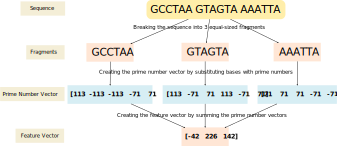
\includegraphics[width=\linewidth]{figures/PrimeNumberScoring.pdf}
  \caption{Example of feature extraction in the PNH}\label{fig:pnh}
\end{figure}

\subsection{Choice of primes for PNH}

The PNH provides a computationally light approach to extract features
from a nucleotide sequence.  Each of the $p$ dimensional features
embody nucleotide frequencies which is sensitive to biologically
meaningful features such as: direct repeats, inverted repeats, and
skew patterns~\cite{hemert-18} but is insensitive to inversions.  This
is the intuition behind the usage of PNH.

The choice of prime numbers to encode nucleotide is a balance.  Small
prime numbers (such as 3, 17, 23, etc.) were avoided in an attempt to
increase the uniqueness of the feature values~\cite{ye-14}.
Conversely, very large values are not used to ensure that a few
differences do not skew the features.  The default values of $P_{A}$ =
113 and $P_{G}$ = 71 were identified via preliminary analysis on HIV
sequences~\cite{delgado-15} and were also used as guidance for the
prime number choices, but was not highly optimized for any particular
organisms' genome.  Moreover, smaller values permit the use of faster,
primitive datatypes without concerns about numeric overflows (within
reason) during summations (see Figure~\ref{fig:pnh}).

\subsection{Impact of hyperparameters}

The Prime Numbers-based Heuristic (PNH) involves two key
hyperparameters, namely -- \ding{182} the number of features $p$ used
for comparing two reads, and \ding{183} $\tau_{prime}$: the threshold
Euclidean distance used to decide if two reads are sufficiently
similar.  Currently, the value of $\tau_{prime}$ for a given reference
sequence is computed as the average Euclidean distance from a given
reference strain minus the standard deviation.

The number of $p$ features has been set to a default value of 4 based
on experimental results summarized in
Figure~\ref{fig:pri-qual}. Overall, the number of features $p$ does
not have a significant impact on the clustering quality -- \ie\/ NMI
and purity do not vary much.  However, as the number of features $p$
is increased the number of clusters increase due to too many
false-negatives as the reads are broken into too short fragments.
Moreover, the memory usage also increases due to the overhead of
storing the large features.  Consequently, in this study, we have set
the value of $p$ to be 4.

\begin{figure}[h]
  \begin{minipage}{\linewidth}
    \centerline{\includegraphics[width=\linewidth]{../charts/param_analysis/primes_features_quality.pdf}}
    \centerline{(a) Impact on quality}
  \end{minipage}
  \begin{minipage}{\linewidth}
    \centerline{\includegraphics[width=\linewidth]{../charts/param_analysis/primes_features_runtime.pdf}}    
    \centerline{(b) Impact on runtime}
  \end{minipage}
  \caption{Impact of varying number of PNH features $p$}\label{fig:pri-qual}
\end{figure}


\section{EXPERIMENTS \& DISCUSSIONS}\label{sec:results}

The effectiveness of the proposed Approximate Spanning Tree (AST) and
the Prime Number based Heuristic (PNH) has been empirically assessed
using two different types of datasets.  The first dataset was
Expressed Sequence Tags (ESTs) from different species as summarized in
Table~\ref{tab:est-ds}.  This dataset consists of characteristic
short reads (about 300 -- 500 nucleotides) that have been used by
several investigators in the past.  

\begin{table}[h]
  \caption{Summary of EST dataset used in experiments}
  \begin{center}
    \begin{tabular}{|l|r|c|r|p{1in}|}
      \hline

      {\bf Name} & {\bf \#Reads} & {\bf Avg Length}     & {\bf Size}  & {\bf Description}  \\
           &         & \bf{(mean$\pm$ SD)} & \bf{(MB)}  &   \\ \hline

      S8   & 150,295 & 300.9$\pm$58 & 48 & Synthetic dataset from ~\cite{james-18} \\ \hline

      C08  & 100,585 & 468.2$\pm$74 & 48 & Synthetic ESTs from ~\cite{hazelhurst-11} \\ \hline

      A076941 & 76,941 & 427.2$\pm$128 & 42 & \emph{Arabidopsis} ESTs from ~\cite{hazelhurst-11} \\ \hline
      
      \hline
    \end{tabular}\label{tab:est-ds}
  \end{center}
\end{table}


\q{S8} is a synthetic data set from James \etal~\cite{james-18}.  The
\q{C08} is a synthetically generated test dataset generated using
ESTsim (see ~\cite{hazelhurst-11} for details).  The \q{A076941}
dataset contains a subset of \emph{Arabidopsis} \emph{Thaliana} ESTs
downloaded from Genbank.  The \q{C08} and \q{A076941} datasets were
primary used because they have been used by Hazelhurst
\etal~\cite{hazelhurst-11} for assessment of \q{wcd-kaboom}.


The second dataset was viral genome fragments summarized in
Table~\ref{tab:virus-ds}.  This datasets consists of \emph{much}
longer reads (1000s of nucleotides) when compared to the EST dataset.
The \q{HA} dataset consists of Haemagglutinin (HA) segments from
multiple Influenza serotypes (H1 -- H19) and should ideally result in
20 clusters.  This dataset has been downloaded from Influenza Research
Database~\cite{bogner-06}.  The \q{Dengue} dataset consists of the
full genome of all 4 serotypes of dengue.  These long genomes are
analogous to the long reads (\mytilde 10,000 bases) produced by the
RSII platform from Pacific bioscience.  It has been downloaded from
Virus Variation Resource~\cite{brister-14}, specifically from the
Virus Pathogen Database~\cite{pickett-12}.  Ideally, this dataset
should generate 4 clusters but due to high homology between the
serotypes, most clustering software yield just 1 cluster.

\begin{table}
  \caption{Summary of Virus dataset used in experiments}
  \begin{center}
    \begin{tabular}{|l|r|c|r|p{1in}|}
      \hline

      {\bf Name} & {\bf \#Reads} & {\bf Avg Length} & {\bf Size}  & {\bf Description}  \\
           &         & {\bf (mean$\pm$ SD)} & {\bf (MB)}  &   \\ \hline

      HA   & 65,069 & 1698.8$\pm$7 & 117 & Influenza Haemmaglutinin  (HA) \\ \hline

      Dengue  & 5,286 & 10,588$\pm$181 & 55 & Degune strains (4 serotypes) \\

      \hline
    \end{tabular}\label{tab:virus-ds}
  \end{center}
\end{table}


\subsection{Experimental Platform}

The experiments reported in this paper have been conducted on a
contemporary compute cluster running PBS.  Each compute node on the
cluster consists of two (dual socket) Intel
Xeon\textsuperscript{\textregistered}\/ CPUs (Gold 6126 @ 2.60 GHz)
with hyperthreading disabled.  Each CPU has 14 cores and 19 MiB of
shared L3 cache.  The cluster runs CentOS 7.5 (Linux kernel version
3.10.  All of the software compiled using GNU Compiler Collection
(GCC) version 6.3.0 at \q{-O2} optimization level.  The timings and
memory usage as been recorded using \q{/usr/bin/time} utility.

\subsection{Design of Experiments}

Prior to conducting experiments, the reads in each of the datasets
were randomly shuffled to eliminate any potential patterns that may be
inherently present when the datasets were downloaded.  Each tool
configuration was run as an independent PBS job with 1 core and 12 GB
of memory reserved for it.  The experimental observations for the EST
data and Virus data are shown in Table~\ref{tab:est} and
Table~\ref{tab:virus}.  In these two tables, the row \q{wcd-kbm}
corresponds to \q{wcd} with \q{kaboom} filter configuration.  The run
time data for \q{wcd-kaboom} includes the time taken to generate
suffix arrays as discussed by Hazelhurst \etal~\cite{hazelhurst-11}.
The row with name \q{MST} shows results for base case \peace\/ run
using its default MST.  The rows labeled \q{AST=1} and \q{AST=0.8}
show results for AST with AST-thresholds set to 1.0 and 0.8
respectively.  The rows with \q{PNH} prefix show results from using
the heuristic along with the default $u/v$ and $t/v$ heuristics in
\peace.

\subsection{Discussions}

The results from various experiments conducted using the EST datasets
from Table~\ref{tab:est-ds} are summarized in Table~\ref{tab:est}.
Similarly, the results for the virus datasets from
Table~\ref{tab:virus-ds} are summarized in Table~\ref{tab:virus}.  The
NMI and purity values have been computed using the clustering
generated by \peace-MST as the reference as discussed in
Section~\ref{sec:metrics}.

For the EST datasets, \q{wcd-kaboom} consistently outperformed
\peace-MST as reported by Hazelhurst \etal~\cite{hazelhurst-11}.
However, as shown by the results, the proposed AST approach was
considerably faster than \peace-MST without much compromise in the
quality in most of the cases.  However, \q{wcd-kaboom} outperformed
the AST approach for two out of the three datasets.  In these
datasets, the performance gains of the AST approach was muted due to
the large number of small clusters -- \ie\/ only a few reads were
similar and hence reads could not be rapidly added to the AST (see
discussion in Section~\ref{sec:ast}).  In other words, Kaboom filter
was more successful at eliminating redundant calls to heuristics and
the heavyweight d2-score generation when compared to AST.  In the case
of the \q{A076941} dataset, a dominant portion of the runtime was
consumed for running the $u/v$ and $t/v$ heuristics.  Analysis of the
runtime behaviors suggests that a threshold based on number of
successful reads would be beneficial here -- \ie\/ once some $s$ reads
below the AST-threshold have been found, stop checking further reads.
We plan to pursue this optimization in the near future to assess its
efficacy.  Some degradation was observed in the \q{C08} case, with the
AST approach generating more clusters.  This results in some
degradation of NMI with respect to \peace-MST, but the NMI of 0.837 is
comparable to \q{wcd}'s 0.847.


\begin{table}
  \caption{Results for EST datasets}
  \begin{center}
    \renewcommand{\arraystretch}{1.1}
    
    \begin{tabular}{|l|l|r|r|r|r|r|}
      
      \hline
      \twocol{\bf Tool info} & {\bf Time} & {\bf RAM} & {\bf \#Clu-} & {\bf NMI} & {\bf Pur-} \\
      \twocol{}          & {\bf (mm:ss)} & \bf{(MB)}   & {\bf sters}  &     & \bf{ity}  \\
      \hline

      \gray
      \multicolumn{7}{|l|}{Dataset: S8 (\mytilde 150K seq)} \\ \hline
      
      \twocol{wcd-kbm} & 1:01 & 787 & 2224 & 0.998 & 1 \\ \hline
      
      \vertpeace

      & MST  & 33:05 & 143 & 2000 & 1 & 1 \\ \cline{2-7}
      
      & AST=1.0 & 0:46 & 163 & 2002 & 0.999 & 1.0 \\ \cline{2-7}

      & AST=0.8 & 01:00 & 163 & 2002 & 0.999 & 1.0 \\ \cline{2-7}
      
      & PNH,AST=1.0 & 01:14 & 178 & 2002 & 0.999 & 1.0 \\ \cline{2-7}

      & PNH,AST=0.8 & 01:08 & 179 & 2001 & 0.999 & 1.0 \\ \hline \hline
      
      %%-----------------------------------------------------------------

      \gray
      \multicolumn{7}{|l|}{Dataset: C08 (\mytilde 100K seq)} \\ \hline

      \twocol{wcd-kbm} & 2:00 & 811 & 5746 & 0.847 & 0.999 \\ \hline
      
      \vertpeace

      & MST  & 18:10 & 12587 & 4552 & 1.0 & 1.0 \\ \cline{2-7}
      
      & AST=1.0 & 2:31 & 2724 & 7350 & 0.837 & 0.999 \\ \cline{2-7}

      & AST=0.8 & 3:31 & 5346 & 6952 & 0.886 & 0.999 \\ \cline{2-7}
      
      & PNH,AST=1.0 & 1:14 & 2723 & 39983 & 0.69 & 0.999 \\ \cline{2-7}


      & PNH,AST=0.8 & 8:41 & 5356 & 39601 & 0.685 & 0.999 \\ \hline \hline

      %%-----------------------------------------------------------------

      \gray
      \multicolumn{7}{|l|}{Dataset: A076941 (\mytilde 76.9K seq)} \\ \hline

      \twocol{wcd-kbm} & 0:45 & 568 & 18817 & 0.965 & 0.998 \\ \hline
      
      \vertpeace

      & MST  & 9:57 & 10576 & 17422 & 1.0 & 1.0 \\ \cline{2-7}
      
      & AST=1.0 & 1:54 & 2711 & 18903 & 0.949 & 0.999 \\ \cline{2-7}

      & AST=0.8 & 3:08 & 2712 & 18759 & 0.953 & 0.999 \\ \cline{2-7}

      & PNH,AST=1.0 & 05:16 & 2719 & 39222 & 0.854 & 1.0 \\ \cline{2-7}
      
      & PNH,AST=0.8 & 05:58 & 2718 & 39025 & 0.858 & 1.0  \\ \hline

    \end{tabular}\label{tab:est}
    \renewcommand{\arraystretch}{1.0}
  \end{center}
\end{table}


The most conspicuous performance improvement was observed in the HA
dataset, where the AST method finished clustering in \mytilde 16
seconds, while \q{wcd-kaboom} and \peace-MST took 149 mins and 930
mins respectively.  This corresponds to a remarkable \textgreater\/
550\texttimes\/ and \textgreater\/ 3400\texttimes\/ performance
improvements!  In the case of the Dengue dataset, the performance
improvement of AST over \q{wcd-kaboom} was \mytilde 90\texttimes.  The
results suggest that the AST method will yield good performance
improvements for datasets with large clusters.

\textbf{An unforeseen benefit}: Our experiments revealed an
interesting unforeseen benefit of the AST method for the HA dataset.
The dataset has 19 different serotypes and a few unclassified
reads. However, the serotypes are highly homologous and hence, the
more accurate MST-based approach results in just 8 clusters.  However,
with the AST approach results in detection of these serotypes as shown
in Table~\ref{tab:virus}.  For example, with a threshold of 0.95, the
AST method generates 20 clusters separating out the serotypes which
could be a desirable result.  This behavior will require further
investigation.

\begin{table}
  \caption{Restuls for Virus datasets}
  \begin{center}
    \renewcommand{\arraystretch}{1.1}
    \begin{tabular}{|l|l|r|r|r|r|r|}
      
      \hline
      \twocol{\bf Tool info} & {\bf Time} & {\bf RAM} & {\bf \#Clu-} & {\bf NMI} & {\bf Pur-} \\
      \twocol{}          & {\bf (mm:ss)} & \bf{(MB)}   & {\bf sters}  &     & \bf{ity}  \\
      \hline

      \gray
      \multicolumn{7}{|l|}{Dataset: HA (\mytilde 65K seq)} \\ \hline
      
      \twocol{wcd-kbm} & 149:55 & 1820 & 28 & 0.566 & 1.0 \\ \hline
      
      \vertpeace

      & MST  & 930:06 & 4198 & 8 & 1.0 & 1.0 \\ \cline{2-7}
      
      & AST=1 &  0:16 & 178 & 26 & 0.63 & 1.0  \\ \cline{2-7}

      & AST=0.8 &  0:27 & 180 & 13 & 0.743 & 1.0 \\ \cline{2-7}
      
      & PNH,AST=1 & 0:13 & 185 & 53 & 0.583 & 1.0  \\ \cline{2-7}

      & PNH,AST=0.8 & 0:17.5 & 185 & 45 & 0.591 & 1.0 \\ \hline \hline
      
      %%-----------------------------------------------------------------

      \gray
      \multicolumn{7}{|l|}{Dataset: Dengue (\mytilde 5.2K seq)} \\ \hline
      
      \twocol{wcd-kbm} & 31:45 & 945 & 1 & 1.0 & 1.0 \\ \hline
      
      \vertpeace

      & MST  & 858:17 & 407 & 1 & 1.0 & 1.0  \\ \cline{2-7}
      
      & AST=1 & 0:21 & 78 & 2 & 0 & 1.0 \\ \cline{2-7}

      & AST=0.8 &  0:27 & 180 & 13 & 0.743 & 1.0 \\ \cline{2-7}
      
      & PNH,AST=1 & 0:11 & 79 & 44 & 0 & 1.0 \\ \cline{2-7}

      & PNH,AST=0.8 & 0:12 & 79 & 45 & 0 & 1.0 \\ \hline

    \end{tabular}\label{tab:virus}
    \renewcommand{\arraystretch}{1.0}
  \end{center}
\end{table}


The Prime Numbers based Heuristic (PNH) was able to further boost
runtime performance in the \q{HA} dataset, but at the cost of
reduction in NMI.  For this dataset prime heuristics was able to
provide another 18\% improvement (see Table~\ref{tab:virus}.  It also
increased performance in the \q{Dengue} dataset by another 50\% with
NMI comparable to AST.  For the datasets having relatively shorter
sequences and a large number of clusters (\ie\/ \q{S8}, \q{C08}, and
\q{A076941}) the PNH was slower.  This is attributed to the additional
computational overhead of the PNH and this overhead is not effectively
amortized. Overall, prime heuristics provided clustering with lower
NMIs, except in the case of \q{S8} dataset.  These results suggested
that the PNH is effective in clustering viral genomic data possessing
highly similar, large nucleotide sequences. This type of clustering
has a several biological applications including analysis of microbial
genome variations, Influenza A subtype identification, and identifying
novel viral strains.

\subsection{Memory consumption}

A drawback inherited from \peace\/ is the increased memory usage for
clustering.  For example, in the case of the \q{C08} dataset, the
default MST-based clustering in \peace\/ consumes over 12 GB of RAM
while the AST approach consumes about 5 GB.  In contrast,
\q{wcd-kaboom} consumes only 26 MB (even when the raw dataset size if
48 MB).  The low memory footprint of \q{wcd-kaboom} is attributed to
the fact that it only maintains the suffix array in memory while
processing 1 read at a time.

The increased memory footprint of \peace\/ arises from 2 factors.
First, \peace\/ experiments were conducted by holding all the reads in
memory.  It does have an option to load reads on-demand, but this
option has not been used to minimize runtime.  The largest fraction of
memory usage arises from the caches maintained by \peace.  The cache
has been implemented using a standard binary heap.  It serves as a
priority queue to identify the next read to be added to the MST/AST.
This cache is pruned, but not aggressively, to reduce runtime.
Performing a periodic, deep pruning of this cache will reduce memory
footprint, but at the cost of some increase in runtime.  In addition,
alternative data structures such as 3-tier heap~\cite{higiro-17} can
be utilized to enable efficient pruning.  We are planning to explore
such enhancements to \peace\/ in the near future.

\section{CONCLUSIONS}

Clustering is a vital processing step for analysis of genomic data.
Several software tools have been proposed to enable fast clustering.
Nevertheless, continued advancement in clustering methods is necessary
to keep pace with the ongoing exponential growth of genomic data.
This study proposed two novel enhancements to an existing clustering
software system called \peace.  The first enhancement was the use of
Approximate Spanning Tree (AST) which enables \emph{much faster}
clustering than the current Minimum Spanning Tree (MST) approach.  In
addition, a novel Prime Numbers based Heuristic (PNH) is also
proposed.  The paper discussed these two enhancements in detail and
presented an empirical analysis of their effectiveness.  The empirical
data was collected from experiments conducted using two different
types of data sets.  Moreover, the paper also presented comparison
against \q{wcd-kaboom}, a \emph{fast}, state-of-the-art clustering
software.

The outcomes of this study show that the AST approach effectively
increase the performance of \peace\/ only for datasets with large
clusters (viral genomic sequences).  In the case of Influenza data
set, a dramatic 550\texttimes\/ performance improvement was observed.
In general, the AST approach did not significantly compromise the
quality of the clustering.  In most cases, the AST method generates
additional clusters, but did not impact purity.  These additional
clusters can be merged, if necessary.

The outcomes also indicate that the Prime Number based Heuristic (PNH)
is a promising approach for further increasing the speed, but only for
clustering long genomic sequences.  A detailed investigation of the
effects of hyperparameter choices for PNH is underway to increase its
broader applicability.  Furthermore, we are planning enhancements to
reduce memory footprint by using multi-tier heaps~\cite{higiro-17}.
Importantly, we plan to explore parallel clustering capabilities of
\peace\/ in conjunction with AST and the PNH.

Rapid clustering of viral and bacterial genomes forming large clusters
will provide insight into the genetic diversity. Viral genotypes such
as Influenza A subtypes can be identified by clustering unidentified
genomic sequences with known genotypes. This type of cluster-based
identification approaches has the potential to detect novel viral
strains by separating them into new clusters which does not consist
any known types.  The improved performance of \peace\/ with AST, with
its default parameter settings and without the need for additional
external tools (such as \q{mkesa} for \q{wcd}), makes it an ideal tool
for use by biologists for clustering large datasets.

\newpage


\section*{ACKNOWLEDGMENT}

We thank Dr. Jens Muller for his help to run experiments on the Red
Hawk compute cluster.  We thank Dr. Scott Hazelhurst for his help with
using \q{wcd} for our experiments.

\section*{AUTHOR CONTRIBUTIONS}


D. M. Rao: A first coauthor, implemented AST and PNH in \peace,
involved in running the experiments, analyzing the data, and writing
the paper.

S. Sreeskandarajan: A first coauthor, designed PNH, involved in
running experiments, analyzing the data, and writing the paper.

C. Liang: Helped with implementation, testing, and analysis of MST
approach in \peace.



%%%%%%%%%%%%%%%%%%%%%%%%%%%%%%%%%%%%%%%%%%%%%%%%%%%%%%%%%%%%%%%%%%%%%%%%%%%%%%%%
\bibliographystyle{abbrv}
\bibliography{main}


\end{document}
